\documentclass[1p]{elsarticle_modified}
%\bibliographystyle{elsarticle-num}

%\usepackage[colorlinks]{hyperref}
%\usepackage{abbrmath_seonhwa} %\Abb, \Ascr, \Acal ,\Abf, \Afrak
\usepackage{amsfonts}
\usepackage{amssymb}
\usepackage{amsmath}
\usepackage{amsthm}
\usepackage{scalefnt}
\usepackage{amsbsy}
\usepackage{kotex}
\usepackage{caption}
\usepackage{subfig}
\usepackage{color}
\usepackage{graphicx}
\usepackage{xcolor} %% white, black, red, green, blue, cyan, magenta, yellow
\usepackage{float}
\usepackage{setspace}
\usepackage{hyperref}

\usepackage{tikz}
\usetikzlibrary{arrows}

\usepackage{multirow}
\usepackage{array} % fixed length table
\usepackage{hhline}

%%%%%%%%%%%%%%%%%%%%%
\makeatletter
\renewcommand*\env@matrix[1][\arraystretch]{%
	\edef\arraystretch{#1}%
	\hskip -\arraycolsep
	\let\@ifnextchar\new@ifnextchar
	\array{*\c@MaxMatrixCols c}}
\makeatother %https://tex.stackexchange.com/questions/14071/how-can-i-increase-the-line-spacing-in-a-matrix
%%%%%%%%%%%%%%%

\usepackage[normalem]{ulem}

\newcommand{\msout}[1]{\ifmmode\text{\sout{\ensuremath{#1}}}\else\sout{#1}\fi}
%SOURCE: \msout is \stkout macro in https://tex.stackexchange.com/questions/20609/strikeout-in-math-mode

\newcommand{\cancel}[1]{
	\ifmmode
	{\color{red}\msout{#1}}
	\else
	{\color{red}\sout{#1}}
	\fi
}

\newcommand{\add}[1]{
	{\color{blue}\uwave{#1}}
}

\newcommand{\replace}[2]{
	\ifmmode
	{\color{red}\msout{#1}}{\color{blue}\uwave{#2}}
	\else
	{\color{red}\sout{#1}}{\color{blue}\uwave{#2}}
	\fi
}

\newcommand{\Sol}{\mathcal{S}} %segment
\newcommand{\D}{D} %diagram
\newcommand{\A}{\mathcal{A}} %arc


%%%%%%%%%%%%%%%%%%%%%%%%%%%%%5 test

\def\sl{\operatorname{\textup{SL}}(2,\Cbb)}
\def\psl{\operatorname{\textup{PSL}}(2,\Cbb)}
\def\quan{\mkern 1mu \triangleright \mkern 1mu}

\theoremstyle{definition}
\newtheorem{thm}{Theorem}[section]
\newtheorem{prop}[thm]{Proposition}
\newtheorem{lem}[thm]{Lemma}
\newtheorem{ques}[thm]{Question}
\newtheorem{cor}[thm]{Corollary}
\newtheorem{defn}[thm]{Definition}
\newtheorem{exam}[thm]{Example}
\newtheorem{rmk}[thm]{Remark}
\newtheorem{alg}[thm]{Algorithm}

\newcommand{\I}{\sqrt{-1}}
\begin{document}

%\begin{frontmatter}
%
%\title{Boundary parabolic representations of knots up to 8 crossings}
%
%%% Group authors per affiliation:
%\author{Yunhi Cho} 
%\address{Department of Mathematics, University of Seoul, Seoul, Korea}
%\ead{yhcho@uos.ac.kr}
%
%
%\author{Seonhwa Kim} %\fnref{s_kim}}
%\address{Center for Geometry and Physics, Institute for Basic Science, Pohang, 37673, Korea}
%\ead{ryeona17@ibs.re.kr}
%
%\author{Hyuk Kim}
%\address{Department of Mathematical Sciences, Seoul National University, Seoul 08826, Korea}
%\ead{hyukkim@snu.ac.kr}
%
%\author{Seokbeom Yoon}
%\address{Department of Mathematical Sciences, Seoul National University, Seoul, 08826,  Korea}
%\ead{sbyoon15@snu.ac.kr}
%
%\begin{abstract}
%We find all boundary parabolic representation of knots up to 8 crossings.
%
%\end{abstract}
%\begin{keyword}
%    \MSC[2010] 57M25 
%\end{keyword}
%
%\end{frontmatter}

%\linenumbers
%\tableofcontents
%
\newcommand\colored[1]{\textcolor{white}{\rule[-0.35ex]{0.8em}{1.4ex}}\kern-0.8em\color{red} #1}%
%\newcommand\colored[1]{\textcolor{white}{ #1}\kern-2.17ex	\textcolor{white}{ #1}\kern-1.81ex	\textcolor{white}{ #1}\kern-2.15ex\color{red}#1	}

{\Large $\underline{12n_{0506}~(K12n_{0506})}$}

\setlength{\tabcolsep}{10pt}
\renewcommand{\arraystretch}{1.6}
\vspace{1cm}\begin{tabular}{m{100pt}>{\centering\arraybackslash}m{274pt}}
\multirow{5}{120pt}{
	\centering
	\includegraphics[width=112pt]{../../../GIT/diagram.site/Diagrams/png/2595_12n_0506.png}\\
\ \ \ A knot diagram\footnotemark}&
\allowdisplaybreaks
\textbf{Linearized knot diagam} \\
\cline{2-2}
 &
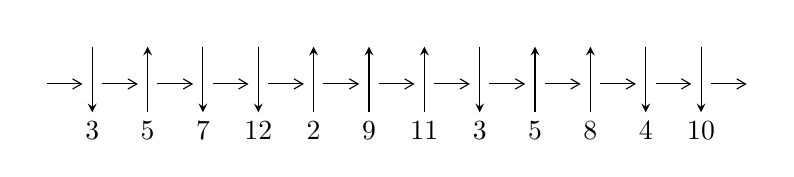
\begin{tikzpicture}[x=20pt, y=17pt]
	% nodes
	\node (C0) at (0, 0) {};
	\node (C1) at (1, 0) {};
	\node (C1U) at (1, +1) {};
	\node (C1D) at (1, -1) {3};

	\node (C2) at (2, 0) {};
	\node (C2U) at (2, +1) {};
	\node (C2D) at (2, -1) {5};

	\node (C3) at (3, 0) {};
	\node (C3U) at (3, +1) {};
	\node (C3D) at (3, -1) {7};

	\node (C4) at (4, 0) {};
	\node (C4U) at (4, +1) {};
	\node (C4D) at (4, -1) {12};

	\node (C5) at (5, 0) {};
	\node (C5U) at (5, +1) {};
	\node (C5D) at (5, -1) {2};

	\node (C6) at (6, 0) {};
	\node (C6U) at (6, +1) {};
	\node (C6D) at (6, -1) {9};

	\node (C7) at (7, 0) {};
	\node (C7U) at (7, +1) {};
	\node (C7D) at (7, -1) {11};

	\node (C8) at (8, 0) {};
	\node (C8U) at (8, +1) {};
	\node (C8D) at (8, -1) {3};

	\node (C9) at (9, 0) {};
	\node (C9U) at (9, +1) {};
	\node (C9D) at (9, -1) {5};

	\node (C10) at (10, 0) {};
	\node (C10U) at (10, +1) {};
	\node (C10D) at (10, -1) {8};

	\node (C11) at (11, 0) {};
	\node (C11U) at (11, +1) {};
	\node (C11D) at (11, -1) {4};

	\node (C12) at (12, 0) {};
	\node (C12U) at (12, +1) {};
	\node (C12D) at (12, -1) {10};
	\node (C13) at (13, 0) {};

	% arrows
	\draw[->,>={angle 60}]
	(C0) edge (C1) (C1) edge (C2) (C2) edge (C3) (C3) edge (C4) (C4) edge (C5) (C5) edge (C6) (C6) edge (C7) (C7) edge (C8) (C8) edge (C9) (C9) edge (C10) (C10) edge (C11) (C11) edge (C12) (C12) edge (C13) ;	\draw[->,>=stealth]
	(C1U) edge (C1D) (C2D) edge (C2U) (C3U) edge (C3D) (C4U) edge (C4D) (C5D) edge (C5U) (C6D) edge (C6U) (C7D) edge (C7U) (C8U) edge (C8D) (C9D) edge (C9U) (C10D) edge (C10U) (C11U) edge (C11D) (C12U) edge (C12D) ;
	\end{tikzpicture} \\
\hhline{~~} \\& 
\textbf{Solving Sequence} \\ \cline{2-2} 
 &
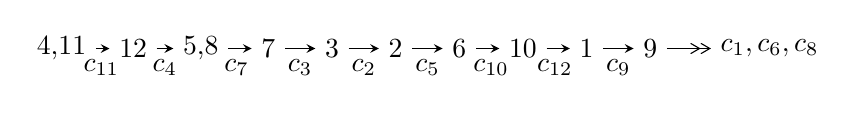
\begin{tikzpicture}[x=23pt, y=7pt]
	% node
	\node (A0) at (-1/8, 0) {4,11};
	\node (A1) at (1, 0) {12};
	\node (A2) at (33/16, 0) {5,8};
	\node (A3) at (25/8, 0) {7};
	\node (A4) at (33/8, 0) {3};
	\node (A5) at (41/8, 0) {2};
	\node (A6) at (49/8, 0) {6};
	\node (A7) at (57/8, 0) {10};
	\node (A8) at (65/8, 0) {1};
	\node (A9) at (73/8, 0) {9};
	\node (C1) at (1/2, -1) {$c_{11}$};
	\node (C2) at (3/2, -1) {$c_{4}$};
	\node (C3) at (21/8, -1) {$c_{7}$};
	\node (C4) at (29/8, -1) {$c_{3}$};
	\node (C5) at (37/8, -1) {$c_{2}$};
	\node (C6) at (45/8, -1) {$c_{5}$};
	\node (C7) at (53/8, -1) {$c_{10}$};
	\node (C8) at (61/8, -1) {$c_{12}$};
	\node (C9) at (69/8, -1) {$c_{9}$};
	\node (A10) at (11, 0) {$c_{1},c_{6},c_{8}$};

	% edge
	\draw[->,>=stealth]	
	(A0) edge (A1) (A1) edge (A2) (A2) edge (A3) (A3) edge (A4) (A4) edge (A5) (A5) edge (A6) (A6) edge (A7) (A7) edge (A8) (A8) edge (A9) ;
	\draw[->>,>={angle 60}]	
	(A9) edge (A10);
\end{tikzpicture} \\ 

\end{tabular} \\

\footnotetext{
The image of knot diagram is generated by the software ``\textbf{Draw programme}" developed by Andrew Bartholomew(\url{http://www.layer8.co.uk/maths/draw/index.htm\#Running-draw}), where we modified some parts for our purpose(\url{https://github.com/CATsTAILs/LinksPainter}).
}\phantom \\ \newline 
\centering \textbf{Ideals for irreducible components\footnotemark of $X_{\text{par}}$} 
 
\begin{align*}
I^u_{1}&=\langle 
-2.92307\times10^{57} u^{49}-8.25153\times10^{56} u^{48}+\cdots+4.65772\times10^{58} b+1.19662\times10^{58},\\
\phantom{I^u_{1}}&\phantom{= \langle  }-3.65030\times10^{58} u^{49}-7.49016\times10^{57} u^{48}+\cdots+9.31544\times10^{58} a-2.43552\times10^{59},\;u^{50}-2 u^{49}+\cdots+4 u-4\rangle \\
I^u_{2}&=\langle 
38499 u^{20}-7436 u^{19}+\cdots+35558 b-156754,\;37681 u^{20}+484 u^{19}+\cdots+35558 a-142970,\\
\phantom{I^u_{2}}&\phantom{= \langle  }u^{21}+u^{20}+\cdots-4 u-4\rangle \\
\\
\end{align*}
\raggedright * 2 irreducible components of $\dim_{\mathbb{C}}=0$, with total 71 representations.\\
\footnotetext{All coefficients of polynomials are rational numbers. But the coefficients are sometimes approximated in decimal forms when there is not enough margin.}
\newpage
\renewcommand{\arraystretch}{1}
\centering \section*{I. $I^u_{1}= \langle -2.92\times10^{57} u^{49}-8.25\times10^{56} u^{48}+\cdots+4.66\times10^{58} b+1.20\times10^{58},\;-3.65\times10^{58} u^{49}-7.49\times10^{57} u^{48}+\cdots+9.32\times10^{58} a-2.44\times10^{59},\;u^{50}-2 u^{49}+\cdots+4 u-4 \rangle$}
\flushleft \textbf{(i) Arc colorings}\\
\begin{tabular}{m{7pt} m{180pt} m{7pt} m{180pt} }
\flushright $a_{4}=$&$\begin{pmatrix}0\\u\end{pmatrix}$ \\
\flushright $a_{11}=$&$\begin{pmatrix}1\\0\end{pmatrix}$ \\
\flushright $a_{12}=$&$\begin{pmatrix}1\\u^2\end{pmatrix}$ \\
\flushright $a_{5}=$&$\begin{pmatrix}- u\\- u^3+u\end{pmatrix}$ \\
\flushright $a_{8}=$&$\begin{pmatrix}0.391855 u^{49}+0.0804058 u^{48}+\cdots+18.2311 u+2.61450\\0.0627575 u^{49}+0.0177158 u^{48}+\cdots+6.02426 u-0.256911\end{pmatrix}$ \\
\flushright $a_{7}=$&$\begin{pmatrix}0.329097 u^{49}+0.0626900 u^{48}+\cdots+12.2069 u+2.87141\\0.0627575 u^{49}+0.0177158 u^{48}+\cdots+6.02426 u-0.256911\end{pmatrix}$ \\
\flushright $a_{3}=$&$\begin{pmatrix}-0.269929 u^{49}+0.335316 u^{48}+\cdots+2.98112 u-9.82945\\0.884089 u^{49}-0.664841 u^{48}+\cdots-6.59794 u+3.47371\end{pmatrix}$ \\
\flushright $a_{2}=$&$\begin{pmatrix}-1.13386 u^{49}+1.13404 u^{48}+\cdots+2.55589 u-12.9459\\0.626077 u^{49}-0.347864 u^{48}+\cdots-5.91190 u+2.87366\end{pmatrix}$ \\
\flushright $a_{6}=$&$\begin{pmatrix}-1.07851 u^{49}+1.75858 u^{48}+\cdots+67.4506 u-7.31372\\-0.837429 u^{49}+0.432036 u^{48}+\cdots-0.0882456 u-3.75890\end{pmatrix}$ \\
\flushright $a_{10}=$&$\begin{pmatrix}1.44758 u^{49}-1.29391 u^{48}+\cdots+7.34620 u-2.10940\\0.579155 u^{49}-0.441145 u^{48}+\cdots-5.55360 u+1.01483\end{pmatrix}$ \\
\flushright $a_{1}=$&$\begin{pmatrix}-0.00688015 u^{49}+1.00008 u^{48}+\cdots+22.7865 u+12.1643\\1.25272 u^{49}-0.864448 u^{48}+\cdots+16.6689 u+2.78210\end{pmatrix}$ \\
\flushright $a_{9}=$&$\begin{pmatrix}1.91394 u^{49}-1.77626 u^{48}+\cdots+6.20475 u-1.13893\\0.783142 u^{49}-0.639256 u^{48}+\cdots-4.34819 u+1.84583\end{pmatrix}$\\&\end{tabular}
\flushleft \textbf{(ii) Obstruction class $= -1$}\\~\\
\flushleft \textbf{(iii) Cusp Shapes $= 1.34948 u^{49}-0.608726 u^{48}+\cdots-1.48538 u-1.03264$}\\~\\
\newpage\renewcommand{\arraystretch}{1}
\flushleft \textbf{(iv) u-Polynomials at the component}\newline \\
\begin{tabular}{m{50pt}|m{274pt}}
Crossings & \hspace{64pt}u-Polynomials at each crossing \\
\hline $$\begin{aligned}c_{1}\end{aligned}$$&$\begin{aligned}
&u^{50}+75 u^{49}+\cdots-199 u+1
\end{aligned}$\\
\hline $$\begin{aligned}c_{2},c_{5}\end{aligned}$$&$\begin{aligned}
&u^{50}+u^{49}+\cdots+37 u-1
\end{aligned}$\\
\hline $$\begin{aligned}c_{3}\end{aligned}$$&$\begin{aligned}
&u^{50}+3 u^{49}+\cdots-622 u+257
\end{aligned}$\\
\hline $$\begin{aligned}c_{4},c_{11}\end{aligned}$$&$\begin{aligned}
&u^{50}+2 u^{49}+\cdots-4 u-4
\end{aligned}$\\
\hline $$\begin{aligned}c_{6}\end{aligned}$$&$\begin{aligned}
&u^{50}+47 u^{48}+\cdots-87532 u-28244
\end{aligned}$\\
\hline $$\begin{aligned}c_{7},c_{10}\end{aligned}$$&$\begin{aligned}
&u^{50}+6 u^{49}+\cdots-82 u-4
\end{aligned}$\\
\hline $$\begin{aligned}c_{8}\end{aligned}$$&$\begin{aligned}
&u^{50}- u^{49}+\cdots+3878700 u+630961
\end{aligned}$\\
\hline $$\begin{aligned}c_{9}\end{aligned}$$&$\begin{aligned}
&u^{50}-2 u^{49}+\cdots-9207 u+307
\end{aligned}$\\
\hline $$\begin{aligned}c_{12}\end{aligned}$$&$\begin{aligned}
&u^{50}-11 u^{49}+\cdots-1988004 u+270187
\end{aligned}$\\
\hline
\end{tabular}\\~\\
\newpage\renewcommand{\arraystretch}{1}
\flushleft \textbf{(v) Riley Polynomials at the component}\newline \\
\begin{tabular}{m{50pt}|m{274pt}}
Crossings & \hspace{64pt}Riley Polynomials at each crossing \\
\hline $$\begin{aligned}c_{1}\end{aligned}$$&$\begin{aligned}
&y^{50}-189 y^{49}+\cdots-22527 y+1
\end{aligned}$\\
\hline $$\begin{aligned}c_{2},c_{5}\end{aligned}$$&$\begin{aligned}
&y^{50}+75 y^{49}+\cdots-199 y+1
\end{aligned}$\\
\hline $$\begin{aligned}c_{3}\end{aligned}$$&$\begin{aligned}
&y^{50}-23 y^{49}+\cdots-130398 y+66049
\end{aligned}$\\
\hline $$\begin{aligned}c_{4},c_{11}\end{aligned}$$&$\begin{aligned}
&y^{50}-42 y^{49}+\cdots+736 y+16
\end{aligned}$\\
\hline $$\begin{aligned}c_{6}\end{aligned}$$&$\begin{aligned}
&y^{50}+94 y^{49}+\cdots-6283430848 y+797723536
\end{aligned}$\\
\hline $$\begin{aligned}c_{7},c_{10}\end{aligned}$$&$\begin{aligned}
&y^{50}+44 y^{49}+\cdots-1100 y+16
\end{aligned}$\\
\hline $$\begin{aligned}c_{8}\end{aligned}$$&$\begin{aligned}
&y^{50}-51 y^{49}+\cdots-6506346297832 y+398111783521
\end{aligned}$\\
\hline $$\begin{aligned}c_{9}\end{aligned}$$&$\begin{aligned}
&y^{50}+84 y^{49}+\cdots-193343697 y+94249
\end{aligned}$\\
\hline $$\begin{aligned}c_{12}\end{aligned}$$&$\begin{aligned}
&y^{50}-67 y^{49}+\cdots+7872728157574 y+73001014969
\end{aligned}$\\
\hline
\end{tabular}\\~\\
\newpage\flushleft \textbf{(vi) Complex Volumes and Cusp Shapes}
$$\begin{array}{c|c|c}  
\text{Solutions to }I^u_{1}& \I (\text{vol} + \sqrt{-1}CS) & \text{Cusp shape}\\
 \hline 
\begin{aligned}
u &= \phantom{-}1.07906\phantom{ +0.000000I} \\
a &= \phantom{-}0.456631\phantom{ +0.000000I} \\
b &= -0.343403\phantom{ +0.000000I}\end{aligned}
 & -1.80303\phantom{ +0.000000I} & -5.94880\phantom{ +0.000000I} \\ \hline\begin{aligned}
u &= \phantom{-}0.648336 + 0.609293 I \\
a &= \phantom{-}0.128763 - 0.334259 I \\
b &= \phantom{-}0.106776 - 0.597923 I\end{aligned}
 & -1.18171 - 1.55259 I & -6.05321 + 2.36458 I \\ \hline\begin{aligned}
u &= \phantom{-}0.648336 - 0.609293 I \\
a &= \phantom{-}0.128763 + 0.334259 I \\
b &= \phantom{-}0.106776 + 0.597923 I\end{aligned}
 & -1.18171 + 1.55259 I & -6.05321 - 2.36458 I \\ \hline\begin{aligned}
u &= \phantom{-}0.811486 + 0.321287 I \\
a &= \phantom{-}0.70261 + 1.71571 I \\
b &= \phantom{-}0.205601 + 0.738871 I\end{aligned}
 & -1.33799 - 1.34735 I & -5.76164 + 1.69141 I \\ \hline\begin{aligned}
u &= \phantom{-}0.811486 - 0.321287 I \\
a &= \phantom{-}0.70261 - 1.71571 I \\
b &= \phantom{-}0.205601 - 0.738871 I\end{aligned}
 & -1.33799 + 1.34735 I & -5.76164 - 1.69141 I \\ \hline\begin{aligned}
u &= -0.104502 + 0.839206 I \\
a &= \phantom{-}0.218390 + 0.701022 I \\
b &= -0.927719 - 0.160877 I\end{aligned}
 & -9.87904 + 3.10011 I & -1.02029 - 2.56068 I \\ \hline\begin{aligned}
u &= -0.104502 - 0.839206 I \\
a &= \phantom{-}0.218390 - 0.701022 I \\
b &= -0.927719 + 0.160877 I\end{aligned}
 & -9.87904 - 3.10011 I & -1.02029 + 2.56068 I \\ \hline\begin{aligned}
u &= -1.16764\phantom{ +0.000000I} \\
a &= \phantom{-}0.705198\phantom{ +0.000000I} \\
b &= \phantom{-}1.36379\phantom{ +0.000000I}\end{aligned}
 & -0.594673\phantom{ +0.000000I} & -14.5600\phantom{ +0.000000I} \\ \hline\begin{aligned}
u &= \phantom{-}0.066997 + 0.819280 I \\
a &= \phantom{-}0.063502 - 0.153656 I \\
b &= \phantom{-}0.279335 - 1.126760 I\end{aligned}
 & -1.19165 - 2.46840 I & \phantom{-}1.22355 + 1.33250 I \\ \hline\begin{aligned}
u &= \phantom{-}0.066997 - 0.819280 I \\
a &= \phantom{-}0.063502 + 0.153656 I \\
b &= \phantom{-}0.279335 + 1.126760 I\end{aligned}
 & -1.19165 + 2.46840 I & \phantom{-}1.22355 - 1.33250 I\\
 \hline 
 \end{array}$$\newpage$$\begin{array}{c|c|c}  
\text{Solutions to }I^u_{1}& \I (\text{vol} + \sqrt{-1}CS) & \text{Cusp shape}\\
 \hline 
\begin{aligned}
u &= \phantom{-}1.210460 + 0.134918 I \\
a &= \phantom{-}0.158769 + 0.327791 I \\
b &= \phantom{-}0.880017 - 0.080173 I\end{aligned}
 & -3.08696 - 0.57146 I & \phantom{-0.000000 } 0 \\ \hline\begin{aligned}
u &= \phantom{-}1.210460 - 0.134918 I \\
a &= \phantom{-}0.158769 - 0.327791 I \\
b &= \phantom{-}0.880017 + 0.080173 I\end{aligned}
 & -3.08696 + 0.57146 I & \phantom{-0.000000 } 0 \\ \hline\begin{aligned}
u &= \phantom{-}0.129091 + 1.253480 I \\
a &= \phantom{-}0.291397 + 0.571233 I \\
b &= -0.021403 + 1.308110 I\end{aligned}
 & -3.97379 - 2.11896 I & \phantom{-0.000000 } 0 \\ \hline\begin{aligned}
u &= \phantom{-}0.129091 - 1.253480 I \\
a &= \phantom{-}0.291397 - 0.571233 I \\
b &= -0.021403 - 1.308110 I\end{aligned}
 & -3.97379 + 2.11896 I & \phantom{-0.000000 } 0 \\ \hline\begin{aligned}
u &= \phantom{-}1.277370 + 0.120815 I \\
a &= -1.23731 - 2.34133 I \\
b &= \phantom{-}0.263155 - 1.360410 I\end{aligned}
 & -7.52184 - 3.28981 I & \phantom{-0.000000 } 0 \\ \hline\begin{aligned}
u &= \phantom{-}1.277370 - 0.120815 I \\
a &= -1.23731 + 2.34133 I \\
b &= \phantom{-}0.263155 + 1.360410 I\end{aligned}
 & -7.52184 + 3.28981 I & \phantom{-0.000000 } 0 \\ \hline\begin{aligned}
u &= -0.270413 + 1.257420 I \\
a &= \phantom{-}0.228850 - 0.640041 I \\
b &= -0.36396 - 1.41166 I\end{aligned}
 & -14.9314 + 7.6930 I & \phantom{-0.000000 } 0 \\ \hline\begin{aligned}
u &= -0.270413 - 1.257420 I \\
a &= \phantom{-}0.228850 + 0.640041 I \\
b &= -0.36396 + 1.41166 I\end{aligned}
 & -14.9314 - 7.6930 I & \phantom{-0.000000 } 0 \\ \hline\begin{aligned}
u &= -1.309520 + 0.061210 I \\
a &= -1.00267 - 3.07061 I \\
b &= -0.114281 - 1.322420 I\end{aligned}
 & -17.4959 + 3.0650 I & \phantom{-0.000000 } 0 \\ \hline\begin{aligned}
u &= -1.309520 - 0.061210 I \\
a &= -1.00267 + 3.07061 I \\
b &= -0.114281 + 1.322420 I\end{aligned}
 & -17.4959 - 3.0650 I & \phantom{-0.000000 } 0\\
 \hline 
 \end{array}$$\newpage$$\begin{array}{c|c|c}  
\text{Solutions to }I^u_{1}& \I (\text{vol} + \sqrt{-1}CS) & \text{Cusp shape}\\
 \hline 
\begin{aligned}
u &= -1.287640 + 0.262760 I \\
a &= \phantom{-}0.161981 - 0.227519 I \\
b &= -0.707113 - 0.093466 I\end{aligned}
 & -4.36735 + 4.61413 I & \phantom{-0.000000 } 0 \\ \hline\begin{aligned}
u &= -1.287640 - 0.262760 I \\
a &= \phantom{-}0.161981 + 0.227519 I \\
b &= -0.707113 + 0.093466 I\end{aligned}
 & -4.36735 - 4.61413 I & \phantom{-0.000000 } 0 \\ \hline\begin{aligned}
u &= -1.328400 + 0.072360 I \\
a &= \phantom{-}0.44568 - 1.71849 I \\
b &= -0.32965 - 1.40593 I\end{aligned}
 & -8.55310 - 0.56867 I & \phantom{-0.000000 } 0 \\ \hline\begin{aligned}
u &= -1.328400 - 0.072360 I \\
a &= \phantom{-}0.44568 + 1.71849 I \\
b &= -0.32965 + 1.40593 I\end{aligned}
 & -8.55310 + 0.56867 I & \phantom{-0.000000 } 0 \\ \hline\begin{aligned}
u &= \phantom{-}1.311730 + 0.308998 I \\
a &= \phantom{-}1.04568 + 1.62480 I \\
b &= -0.112849 + 1.208320 I\end{aligned}
 & -5.28912 - 1.66036 I & \phantom{-0.000000 } 0 \\ \hline\begin{aligned}
u &= \phantom{-}1.311730 - 0.308998 I \\
a &= \phantom{-}1.04568 - 1.62480 I \\
b &= -0.112849 - 1.208320 I\end{aligned}
 & -5.28912 + 1.66036 I & \phantom{-0.000000 } 0 \\ \hline\begin{aligned}
u &= \phantom{-}1.346080 + 0.075442 I \\
a &= -0.20642 - 1.73825 I \\
b &= -0.88688 - 1.61634 I\end{aligned}
 & -18.0336 + 1.1028 I & \phantom{-0.000000 } 0 \\ \hline\begin{aligned}
u &= \phantom{-}1.346080 - 0.075442 I \\
a &= -0.20642 + 1.73825 I \\
b &= -0.88688 + 1.61634 I\end{aligned}
 & -18.0336 - 1.1028 I & \phantom{-0.000000 } 0 \\ \hline\begin{aligned}
u &= -1.279240 + 0.427359 I \\
a &= -0.775969 - 0.823176 I \\
b &= -0.321757 + 0.101254 I\end{aligned}
 & -13.45950 + 1.53340 I & \phantom{-0.000000 } 0 \\ \hline\begin{aligned}
u &= -1.279240 - 0.427359 I \\
a &= -0.775969 + 0.823176 I \\
b &= -0.321757 - 0.101254 I\end{aligned}
 & -13.45950 - 1.53340 I & \phantom{-0.000000 } 0\\
 \hline 
 \end{array}$$\newpage$$\begin{array}{c|c|c}  
\text{Solutions to }I^u_{1}& \I (\text{vol} + \sqrt{-1}CS) & \text{Cusp shape}\\
 \hline 
\begin{aligned}
u &= -1.331940 + 0.309177 I \\
a &= -0.48326 + 1.82025 I \\
b &= \phantom{-}0.50826 + 1.45369 I\end{aligned}
 & -5.66081 + 6.42848 I & \phantom{-0.000000 } 0 \\ \hline\begin{aligned}
u &= -1.331940 - 0.309177 I \\
a &= -0.48326 - 1.82025 I \\
b &= \phantom{-}0.50826 - 1.45369 I\end{aligned}
 & -5.66081 - 6.42848 I & \phantom{-0.000000 } 0 \\ \hline\begin{aligned}
u &= \phantom{-}1.349410 + 0.336328 I \\
a &= -0.525442 + 0.560601 I \\
b &= -1.37321 + 0.35227 I\end{aligned}
 & -14.4886 - 7.2876 I & \phantom{-0.000000 } 0 \\ \hline\begin{aligned}
u &= \phantom{-}1.349410 - 0.336328 I \\
a &= -0.525442 - 0.560601 I \\
b &= -1.37321 - 0.35227 I\end{aligned}
 & -14.4886 + 7.2876 I & \phantom{-0.000000 } 0 \\ \hline\begin{aligned}
u &= \phantom{-}0.082394 + 0.547321 I \\
a &= \phantom{-}0.986098 - 0.631149 I \\
b &= -0.170671 - 0.044166 I\end{aligned}
 & -0.14617 - 1.49325 I & -0.46873 + 5.87257 I \\ \hline\begin{aligned}
u &= \phantom{-}0.082394 - 0.547321 I \\
a &= \phantom{-}0.986098 + 0.631149 I \\
b &= -0.170671 + 0.044166 I\end{aligned}
 & -0.14617 + 1.49325 I & -0.46873 - 5.87257 I \\ \hline\begin{aligned}
u &= -0.414715 + 0.288195 I \\
a &= \phantom{-}0.101777 + 1.365910 I \\
b &= \phantom{-}0.631123 + 0.377678 I\end{aligned}
 & \phantom{-}1.14736 + 1.01845 I & \phantom{-}7.01184 - 3.19514 I \\ \hline\begin{aligned}
u &= -0.414715 - 0.288195 I \\
a &= \phantom{-}0.101777 - 1.365910 I \\
b &= \phantom{-}0.631123 - 0.377678 I\end{aligned}
 & \phantom{-}1.14736 - 1.01845 I & \phantom{-}7.01184 + 3.19514 I \\ \hline\begin{aligned}
u &= -1.43825 + 0.45806 I \\
a &= \phantom{-}0.93844 - 1.62626 I \\
b &= -0.247398 - 1.377560 I\end{aligned}
 & -9.15198 + 7.96076 I & \phantom{-0.000000 } 0 \\ \hline\begin{aligned}
u &= -1.43825 - 0.45806 I \\
a &= \phantom{-}0.93844 + 1.62626 I \\
b &= -0.247398 + 1.377560 I\end{aligned}
 & -9.15198 - 7.96076 I & \phantom{-0.000000 } 0\\
 \hline 
 \end{array}$$\newpage$$\begin{array}{c|c|c}  
\text{Solutions to }I^u_{1}& \I (\text{vol} + \sqrt{-1}CS) & \text{Cusp shape}\\
 \hline 
\begin{aligned}
u &= \phantom{-}1.50629 + 0.48152 I \\
a &= \phantom{-}0.63158 + 1.81709 I \\
b &= -0.49334 + 1.56307 I\end{aligned}
 & \phantom{-}18.8663 - 13.7470 I & \phantom{-0.000000 } 0 \\ \hline\begin{aligned}
u &= \phantom{-}1.50629 - 0.48152 I \\
a &= \phantom{-}0.63158 - 1.81709 I \\
b &= -0.49334 - 1.56307 I\end{aligned}
 & \phantom{-}18.8663 + 13.7470 I & \phantom{-0.000000 } 0 \\ \hline\begin{aligned}
u &= \phantom{-}1.50100 + 0.52835 I \\
a &= -0.44313 - 1.51722 I \\
b &= \phantom{-}0.24879 - 1.45359 I\end{aligned}
 & -8.62936 - 4.54432 I & \phantom{-0.000000 } 0 \\ \hline\begin{aligned}
u &= \phantom{-}1.50100 - 0.52835 I \\
a &= -0.44313 + 1.51722 I \\
b &= \phantom{-}0.24879 + 1.45359 I\end{aligned}
 & -8.62936 + 4.54432 I & \phantom{-0.000000 } 0 \\ \hline\begin{aligned}
u &= \phantom{-}0.121767 + 0.292619 I \\
a &= -0.22430 - 2.50528 I \\
b &= \phantom{-}0.063783 + 1.250300 I\end{aligned}
 & -3.84376 + 1.74410 I & -5.80851 - 2.56777 I \\ \hline\begin{aligned}
u &= \phantom{-}0.121767 - 0.292619 I \\
a &= -0.22430 + 2.50528 I \\
b &= \phantom{-}0.063783 - 1.250300 I\end{aligned}
 & -3.84376 - 1.74410 I & -5.80851 + 2.56777 I \\ \hline\begin{aligned}
u &= -1.49544 + 0.79557 I \\
a &= -0.698551 + 1.169030 I \\
b &= -0.131534 + 1.396950 I\end{aligned}
 & -18.4852 - 0.1786 I & \phantom{-0.000000 } 0 \\ \hline\begin{aligned}
u &= -1.49544 - 0.79557 I \\
a &= -0.698551 - 1.169030 I \\
b &= -0.131534 - 1.396950 I\end{aligned}
 & -18.4852 + 0.1786 I & \phantom{-0.000000 } 0 \\ \hline\begin{aligned}
u &= -0.058061 + 0.206058 I \\
a &= \phantom{-}4.91262 + 4.09459 I \\
b &= -0.49528 + 1.32653 I\end{aligned}
 & -13.42200 - 2.14669 I & -3.56304 + 0.04666 I \\ \hline\begin{aligned}
u &= -0.058061 - 0.206058 I \\
a &= \phantom{-}4.91262 - 4.09459 I \\
b &= -0.49528 - 1.32653 I\end{aligned}
 & -13.42200 + 2.14669 I & -3.56304 - 0.04666 I\\
 \hline 
 \end{array}$$\newpage\newpage\renewcommand{\arraystretch}{1}
\centering \section*{II. $I^u_{2}= \langle 38499 u^{20}-7436 u^{19}+\cdots+35558 b-156754,\;37681 u^{20}+484 u^{19}+\cdots+35558 a-142970,\;u^{21}+u^{20}+\cdots-4 u-4 \rangle$}
\flushleft \textbf{(i) Arc colorings}\\
\begin{tabular}{m{7pt} m{180pt} m{7pt} m{180pt} }
\flushright $a_{4}=$&$\begin{pmatrix}0\\u\end{pmatrix}$ \\
\flushright $a_{11}=$&$\begin{pmatrix}1\\0\end{pmatrix}$ \\
\flushright $a_{12}=$&$\begin{pmatrix}1\\u^2\end{pmatrix}$ \\
\flushright $a_{5}=$&$\begin{pmatrix}- u\\- u^3+u\end{pmatrix}$ \\
\flushright $a_{8}=$&$\begin{pmatrix}-1.05971 u^{20}-0.0136116 u^{19}+\cdots+4.51401 u+4.02075\\-1.08271 u^{20}+0.209123 u^{19}+\cdots+1.96665 u+4.40840\end{pmatrix}$ \\
\flushright $a_{7}=$&$\begin{pmatrix}0.0230047 u^{20}-0.222735 u^{19}+\cdots+2.54736 u-0.387648\\-1.08271 u^{20}+0.209123 u^{19}+\cdots+1.96665 u+4.40840\end{pmatrix}$ \\
\flushright $a_{3}=$&$\begin{pmatrix}0.723649 u^{20}-0.307821 u^{19}+\cdots-1.97356 u-1.22588\\0.0756229 u^{20}-0.244418 u^{19}+\cdots-0.692727 u+0.527645\end{pmatrix}$ \\
\flushright $a_{2}=$&$\begin{pmatrix}0.714902 u^{20}+0.122827 u^{19}+\cdots-0.881546 u-2.17386\\-1.16677 u^{20}+0.221047 u^{19}+\cdots-0.0621520 u+3.23320\end{pmatrix}$ \\
\flushright $a_{6}=$&$\begin{pmatrix}-0.340767 u^{20}+0.344592 u^{19}+\cdots+2.83759 u+0.174982\\-0.372968 u^{20}+0.0989088 u^{19}+\cdots+0.383767 u+2.08679\end{pmatrix}$ \\
\flushright $a_{10}=$&$\begin{pmatrix}-0.690885 u^{20}+0.802337 u^{19}+\cdots+3.67549 u+2.22392\\-0.822797 u^{20}+0.594803 u^{19}+\cdots+2.71444 u+3.44429\end{pmatrix}$ \\
\flushright $a_{1}=$&$\begin{pmatrix}-0.372659 u^{20}+0.935767 u^{19}+\cdots+0.0702233 u+0.387198\\-0.877608 u^{20}+1.04604 u^{19}+\cdots+1.58693 u+0.580629\end{pmatrix}$ \\
\flushright $a_{9}=$&$\begin{pmatrix}-0.950799 u^{20}+0.416657 u^{19}+\cdots+2.92770 u+2.18803\\-0.476152 u^{20}+0.150515 u^{19}+\cdots+1.91951 u+2.97711\end{pmatrix}$\\&\end{tabular}
\flushleft \textbf{(ii) Obstruction class $= 1$}\\~\\
\flushleft \textbf{(iii) Cusp Shapes $= \frac{19570}{17779} u^{20}+\frac{17174}{17779} u^{19}+\cdots+\frac{45070}{17779} u-\frac{25746}{17779}$}\\~\\
\newpage\renewcommand{\arraystretch}{1}
\flushleft \textbf{(iv) u-Polynomials at the component}\newline \\
\begin{tabular}{m{50pt}|m{274pt}}
Crossings & \hspace{64pt}u-Polynomials at each crossing \\
\hline $$\begin{aligned}c_{1}\end{aligned}$$&$\begin{aligned}
&u^{21}-24 u^{20}+\cdots+16 u+1
\end{aligned}$\\
\hline $$\begin{aligned}c_{2}\end{aligned}$$&$\begin{aligned}
&u^{21}+12 u^{19}+\cdots-4 u-1
\end{aligned}$\\
\hline $$\begin{aligned}c_{3}\end{aligned}$$&$\begin{aligned}
&u^{21}+2 u^{20}+\cdots+u-7
\end{aligned}$\\
\hline $$\begin{aligned}c_{4}\end{aligned}$$&$\begin{aligned}
&u^{21}- u^{20}+\cdots-4 u+4
\end{aligned}$\\
\hline $$\begin{aligned}c_{5}\end{aligned}$$&$\begin{aligned}
&u^{21}+12 u^{19}+\cdots-4 u+1
\end{aligned}$\\
\hline $$\begin{aligned}c_{6}\end{aligned}$$&$\begin{aligned}
&u^{21}- u^{20}+\cdots+20 u+4
\end{aligned}$\\
\hline $$\begin{aligned}c_{7}\end{aligned}$$&$\begin{aligned}
&u^{21}+5 u^{20}+\cdots+34 u+4
\end{aligned}$\\
\hline $$\begin{aligned}c_{8}\end{aligned}$$&$\begin{aligned}
&u^{21}-3 u^{19}+\cdots+5 u+1
\end{aligned}$\\
\hline $$\begin{aligned}c_{9}\end{aligned}$$&$\begin{aligned}
&u^{21}+u^{20}+\cdots+2 u-1
\end{aligned}$\\
\hline $$\begin{aligned}c_{10}\end{aligned}$$&$\begin{aligned}
&u^{21}-5 u^{20}+\cdots+34 u-4
\end{aligned}$\\
\hline $$\begin{aligned}c_{11}\end{aligned}$$&$\begin{aligned}
&u^{21}+u^{20}+\cdots-4 u-4
\end{aligned}$\\
\hline $$\begin{aligned}c_{12}\end{aligned}$$&$\begin{aligned}
&u^{21}-2 u^{20}+\cdots+47 u+7
\end{aligned}$\\
\hline
\end{tabular}\\~\\
\newpage\renewcommand{\arraystretch}{1}
\flushleft \textbf{(v) Riley Polynomials at the component}\newline \\
\begin{tabular}{m{50pt}|m{274pt}}
Crossings & \hspace{64pt}Riley Polynomials at each crossing \\
\hline $$\begin{aligned}c_{1}\end{aligned}$$&$\begin{aligned}
&y^{21}-44 y^{20}+\cdots+232 y-1
\end{aligned}$\\
\hline $$\begin{aligned}c_{2},c_{5}\end{aligned}$$&$\begin{aligned}
&y^{21}+24 y^{20}+\cdots+16 y-1
\end{aligned}$\\
\hline $$\begin{aligned}c_{3}\end{aligned}$$&$\begin{aligned}
&y^{21}-6 y^{20}+\cdots+239 y-49
\end{aligned}$\\
\hline $$\begin{aligned}c_{4},c_{11}\end{aligned}$$&$\begin{aligned}
&y^{21}-17 y^{20}+\cdots-32 y-16
\end{aligned}$\\
\hline $$\begin{aligned}c_{6}\end{aligned}$$&$\begin{aligned}
&y^{21}+19 y^{20}+\cdots+352 y-16
\end{aligned}$\\
\hline $$\begin{aligned}c_{7},c_{10}\end{aligned}$$&$\begin{aligned}
&y^{21}+17 y^{20}+\cdots+12 y-16
\end{aligned}$\\
\hline $$\begin{aligned}c_{8}\end{aligned}$$&$\begin{aligned}
&y^{21}-6 y^{20}+\cdots+29 y-1
\end{aligned}$\\
\hline $$\begin{aligned}c_{9}\end{aligned}$$&$\begin{aligned}
&y^{21}+13 y^{20}+\cdots+6 y-1
\end{aligned}$\\
\hline $$\begin{aligned}c_{12}\end{aligned}$$&$\begin{aligned}
&y^{21}-14 y^{20}+\cdots+67 y-49
\end{aligned}$\\
\hline
\end{tabular}\\~\\
\newpage\flushleft \textbf{(vi) Complex Volumes and Cusp Shapes}
$$\begin{array}{c|c|c}  
\text{Solutions to }I^u_{2}& \I (\text{vol} + \sqrt{-1}CS) & \text{Cusp shape}\\
 \hline 
\begin{aligned}
u &= \phantom{-}0.053654 + 0.994034 I \\
a &= -0.118262 - 0.157903 I \\
b &= \phantom{-}0.261258 - 1.096940 I\end{aligned}
 & -1.82196 - 3.31723 I & -3.56279 + 6.27419 I \\ \hline\begin{aligned}
u &= \phantom{-}0.053654 - 0.994034 I \\
a &= -0.118262 + 0.157903 I \\
b &= \phantom{-}0.261258 + 1.096940 I\end{aligned}
 & -1.82196 + 3.31723 I & -3.56279 - 6.27419 I \\ \hline\begin{aligned}
u &= -1.006310 + 0.386972 I \\
a &= -0.001299 - 0.196953 I \\
b &= -0.510619 - 1.094680 I\end{aligned}
 & -14.5544 + 3.5199 I & -7.00930 - 3.34595 I \\ \hline\begin{aligned}
u &= -1.006310 - 0.386972 I \\
a &= -0.001299 + 0.196953 I \\
b &= -0.510619 + 1.094680 I\end{aligned}
 & -14.5544 - 3.5199 I & -7.00930 + 3.34595 I \\ \hline\begin{aligned}
u &= \phantom{-}1.07842\phantom{ +0.000000I} \\
a &= \phantom{-}0.535095\phantom{ +0.000000I} \\
b &= \phantom{-}1.10310\phantom{ +0.000000I}\end{aligned}
 & -0.187749\phantom{ +0.000000I} & \phantom{-}6.00000\phantom{ +0.000000I} \\ \hline\begin{aligned}
u &= \phantom{-}0.727444 + 0.493982 I \\
a &= -0.187671 - 0.933435 I \\
b &= \phantom{-}0.329896 - 0.180152 I\end{aligned}
 & -0.14218 - 1.80240 I & \phantom{-}2.07850 + 4.52264 I \\ \hline\begin{aligned}
u &= \phantom{-}0.727444 - 0.493982 I \\
a &= -0.187671 + 0.933435 I \\
b &= \phantom{-}0.329896 + 0.180152 I\end{aligned}
 & -0.14218 + 1.80240 I & \phantom{-}2.07850 - 4.52264 I \\ \hline\begin{aligned}
u &= \phantom{-}0.712915 + 0.901061 I \\
a &= \phantom{-}0.383343 + 0.651191 I \\
b &= \phantom{-}0.098075 + 1.273330 I\end{aligned}
 & -3.65276 - 0.25703 I & -6.52769 - 0.27177 I \\ \hline\begin{aligned}
u &= \phantom{-}0.712915 - 0.901061 I \\
a &= \phantom{-}0.383343 - 0.651191 I \\
b &= \phantom{-}0.098075 - 1.273330 I\end{aligned}
 & -3.65276 + 0.25703 I & -6.52769 + 0.27177 I \\ \hline\begin{aligned}
u &= \phantom{-}1.239990 + 0.303227 I \\
a &= -0.83651 - 2.17539 I \\
b &= \phantom{-}0.22167 - 1.41775 I\end{aligned}
 & -5.86381 - 4.09879 I & -5.03465 + 3.45560 I\\
 \hline 
 \end{array}$$\newpage$$\begin{array}{c|c|c}  
\text{Solutions to }I^u_{2}& \I (\text{vol} + \sqrt{-1}CS) & \text{Cusp shape}\\
 \hline 
\begin{aligned}
u &= \phantom{-}1.239990 - 0.303227 I \\
a &= -0.83651 + 2.17539 I \\
b &= \phantom{-}0.22167 + 1.41775 I\end{aligned}
 & -5.86381 + 4.09879 I & -5.03465 - 3.45560 I \\ \hline\begin{aligned}
u &= -1.261550 + 0.269071 I \\
a &= -0.62409 + 2.26542 I \\
b &= -0.366033 + 1.347970 I\end{aligned}
 & -15.6653 - 0.5794 I & -6.15872 - 0.08532 I \\ \hline\begin{aligned}
u &= -1.261550 - 0.269071 I \\
a &= -0.62409 - 2.26542 I \\
b &= -0.366033 - 1.347970 I\end{aligned}
 & -15.6653 + 0.5794 I & -6.15872 + 0.08532 I \\ \hline\begin{aligned}
u &= -1.279400 + 0.192903 I \\
a &= \phantom{-}0.332530 - 0.511316 I \\
b &= \phantom{-}1.066330 - 0.560224 I\end{aligned}
 & -3.93246 + 2.61822 I & -7.09974 - 2.69906 I \\ \hline\begin{aligned}
u &= -1.279400 - 0.192903 I \\
a &= \phantom{-}0.332530 + 0.511316 I \\
b &= \phantom{-}1.066330 + 0.560224 I\end{aligned}
 & -3.93246 - 2.61822 I & -7.09974 + 2.69906 I \\ \hline\begin{aligned}
u &= \phantom{-}1.348700 + 0.186645 I \\
a &= \phantom{-}1.03417 + 1.35712 I \\
b &= -0.146518 + 1.073210 I\end{aligned}
 & -6.54748 - 0.69924 I & -7.57202 - 0.34785 I \\ \hline\begin{aligned}
u &= \phantom{-}1.348700 - 0.186645 I \\
a &= \phantom{-}1.03417 - 1.35712 I \\
b &= -0.146518 - 1.073210 I\end{aligned}
 & -6.54748 + 0.69924 I & -7.57202 + 0.34785 I \\ \hline\begin{aligned}
u &= -1.41010 + 0.39622 I \\
a &= -0.58101 + 1.57427 I \\
b &= \phantom{-}0.498672 + 1.276340 I\end{aligned}
 & -6.71074 + 8.26508 I & -4.78242 - 6.51636 I \\ \hline\begin{aligned}
u &= -1.41010 - 0.39622 I \\
a &= -0.58101 - 1.57427 I \\
b &= \phantom{-}0.498672 - 1.276340 I\end{aligned}
 & -6.71074 - 8.26508 I & -4.78242 + 6.51636 I \\ \hline\begin{aligned}
u &= -0.164557 + 0.384273 I \\
a &= -0.66874 + 2.46746 I \\
b &= \phantom{-}0.495722 + 0.644048 I\end{aligned}
 & -0.232681 - 0.315786 I & -1.33114 - 1.22918 I\\
 \hline 
 \end{array}$$\newpage$$\begin{array}{c|c|c}  
\text{Solutions to }I^u_{2}& \I (\text{vol} + \sqrt{-1}CS) & \text{Cusp shape}\\
 \hline 
\begin{aligned}
u &= -0.164557 - 0.384273 I \\
a &= -0.66874 - 2.46746 I \\
b &= \phantom{-}0.495722 - 0.644048 I\end{aligned}
 & -0.232681 + 0.315786 I & -1.33114 + 1.22918 I\\
 \hline 
 \end{array}$$\newpage
\newpage\renewcommand{\arraystretch}{1}
\centering \section*{ III. u-Polynomials}
\begin{tabular}{m{50pt}|m{274pt}}
Crossings & \hspace{64pt}u-Polynomials at each crossing \\
\hline $$\begin{aligned}c_{1}\end{aligned}$$&$\begin{aligned}
&(u^{21}-24 u^{20}+\cdots+16 u+1)(u^{50}+75 u^{49}+\cdots-199 u+1)
\end{aligned}$\\
\hline $$\begin{aligned}c_{2}\end{aligned}$$&$\begin{aligned}
&(u^{21}+12 u^{19}+\cdots-4 u-1)(u^{50}+u^{49}+\cdots+37 u-1)
\end{aligned}$\\
\hline $$\begin{aligned}c_{3}\end{aligned}$$&$\begin{aligned}
&(u^{21}+2 u^{20}+\cdots+u-7)(u^{50}+3 u^{49}+\cdots-622 u+257)
\end{aligned}$\\
\hline $$\begin{aligned}c_{4}\end{aligned}$$&$\begin{aligned}
&(u^{21}- u^{20}+\cdots-4 u+4)(u^{50}+2 u^{49}+\cdots-4 u-4)
\end{aligned}$\\
\hline $$\begin{aligned}c_{5}\end{aligned}$$&$\begin{aligned}
&(u^{21}+12 u^{19}+\cdots-4 u+1)(u^{50}+u^{49}+\cdots+37 u-1)
\end{aligned}$\\
\hline $$\begin{aligned}c_{6}\end{aligned}$$&$\begin{aligned}
&(u^{21}- u^{20}+\cdots+20 u+4)(u^{50}+47 u^{48}+\cdots-87532 u-28244)
\end{aligned}$\\
\hline $$\begin{aligned}c_{7}\end{aligned}$$&$\begin{aligned}
&(u^{21}+5 u^{20}+\cdots+34 u+4)(u^{50}+6 u^{49}+\cdots-82 u-4)
\end{aligned}$\\
\hline $$\begin{aligned}c_{8}\end{aligned}$$&$\begin{aligned}
&(u^{21}-3 u^{19}+\cdots+5 u+1)(u^{50}- u^{49}+\cdots+3878700 u+630961)
\end{aligned}$\\
\hline $$\begin{aligned}c_{9}\end{aligned}$$&$\begin{aligned}
&(u^{21}+u^{20}+\cdots+2 u-1)(u^{50}-2 u^{49}+\cdots-9207 u+307)
\end{aligned}$\\
\hline $$\begin{aligned}c_{10}\end{aligned}$$&$\begin{aligned}
&(u^{21}-5 u^{20}+\cdots+34 u-4)(u^{50}+6 u^{49}+\cdots-82 u-4)
\end{aligned}$\\
\hline $$\begin{aligned}c_{11}\end{aligned}$$&$\begin{aligned}
&(u^{21}+u^{20}+\cdots-4 u-4)(u^{50}+2 u^{49}+\cdots-4 u-4)
\end{aligned}$\\
\hline $$\begin{aligned}c_{12}\end{aligned}$$&$\begin{aligned}
&(u^{21}-2 u^{20}+\cdots+47 u+7)(u^{50}-11 u^{49}+\cdots-1988004 u+270187)
\end{aligned}$\\
\hline
\end{tabular}\newpage\renewcommand{\arraystretch}{1}
\centering \section*{ IV. Riley Polynomials}
\begin{tabular}{m{50pt}|m{274pt}}
Crossings & \hspace{64pt}Riley Polynomials at each crossing \\
\hline $$\begin{aligned}c_{1}\end{aligned}$$&$\begin{aligned}
&(y^{21}-44 y^{20}+\cdots+232 y-1)(y^{50}-189 y^{49}+\cdots-22527 y+1)
\end{aligned}$\\
\hline $$\begin{aligned}c_{2},c_{5}\end{aligned}$$&$\begin{aligned}
&(y^{21}+24 y^{20}+\cdots+16 y-1)(y^{50}+75 y^{49}+\cdots-199 y+1)
\end{aligned}$\\
\hline $$\begin{aligned}c_{3}\end{aligned}$$&$\begin{aligned}
&(y^{21}-6 y^{20}+\cdots+239 y-49)(y^{50}-23 y^{49}+\cdots-130398 y+66049)
\end{aligned}$\\
\hline $$\begin{aligned}c_{4},c_{11}\end{aligned}$$&$\begin{aligned}
&(y^{21}-17 y^{20}+\cdots-32 y-16)(y^{50}-42 y^{49}+\cdots+736 y+16)
\end{aligned}$\\
\hline $$\begin{aligned}c_{6}\end{aligned}$$&$\begin{aligned}
&(y^{21}+19 y^{20}+\cdots+352 y-16)\\
&\cdot(y^{50}+94 y^{49}+\cdots-6283430848 y+797723536)
\end{aligned}$\\
\hline $$\begin{aligned}c_{7},c_{10}\end{aligned}$$&$\begin{aligned}
&(y^{21}+17 y^{20}+\cdots+12 y-16)(y^{50}+44 y^{49}+\cdots-1100 y+16)
\end{aligned}$\\
\hline $$\begin{aligned}c_{8}\end{aligned}$$&$\begin{aligned}
&(y^{21}-6 y^{20}+\cdots+29 y-1)\\
&\cdot(y^{50}-51 y^{49}+\cdots-6506346297832 y+398111783521)
\end{aligned}$\\
\hline $$\begin{aligned}c_{9}\end{aligned}$$&$\begin{aligned}
&(y^{21}+13 y^{20}+\cdots+6 y-1)\\
&\cdot(y^{50}+84 y^{49}+\cdots-193343697 y+94249)
\end{aligned}$\\
\hline $$\begin{aligned}c_{12}\end{aligned}$$&$\begin{aligned}
&(y^{21}-14 y^{20}+\cdots+67 y-49)\\
&\cdot(y^{50}-67 y^{49}+\cdots+7872728157574 y+73001014969)
\end{aligned}$\\
\hline
\end{tabular}
\vskip 2pc
\end{document}